%-----------------------------------------------------------------
%	GEOGRAPHIC ANALYSIS
%	!TEX root = ./../main.tex
%-----------------------------------------------------------------
\subsection{Analysis of the location}
A particularly important variable in this analysis is, obviously, the location of genesis of the storms, and possibly their location of death.

In this part we do an exploratory comparison of the difference in position of genesis and death of tropical-cyclones between low-SST and high-SST years.

\medskip
In \Cref{fig:natl-positions} we can see the distributions of genesis and death positions (longitude and latitde) of the storms occurred on the North Atlantic basin, while in \Cref{tab:natl-positions} we can see the expected value of the distributions.

The results suggest show the major difference between low-SST and high-SST years is the location of the genesis of the hurricanes, as it seems to be displaced to the South-East. However, there is no significant difference in the death location.
\begin{figure}[H]
	\centering
	\subfloat[Distribution of the genesis longitude]{%
		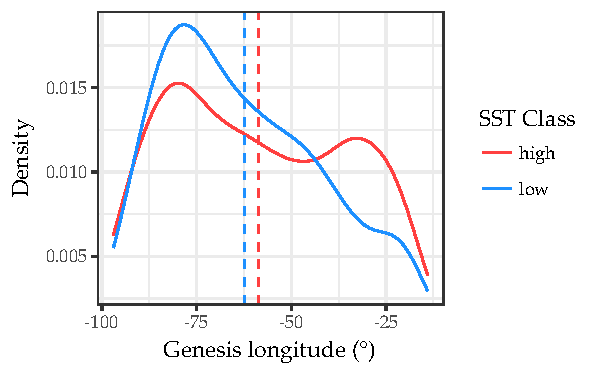
\includegraphics[width=0.5\textwidth]{./images/natl-init-long}
		\label{fig:images/natl-init-long}%
		}%
	\subfloat[Distribution of the death longitude]{%
		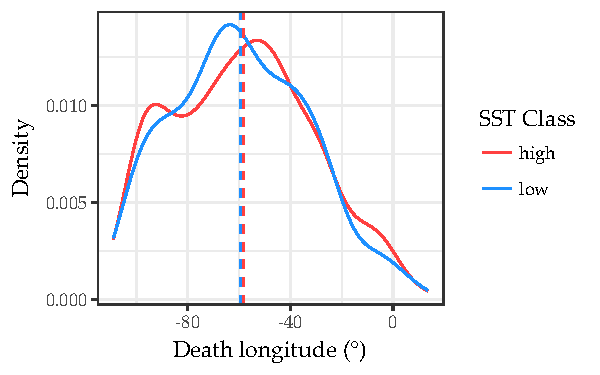
\includegraphics[width=0.5\textwidth]{./images/natl-final-long}
		\label{fig:images/natl-final-long}%
		}%
	\\
	\subfloat[Distribution of the genesis latitude]{%
		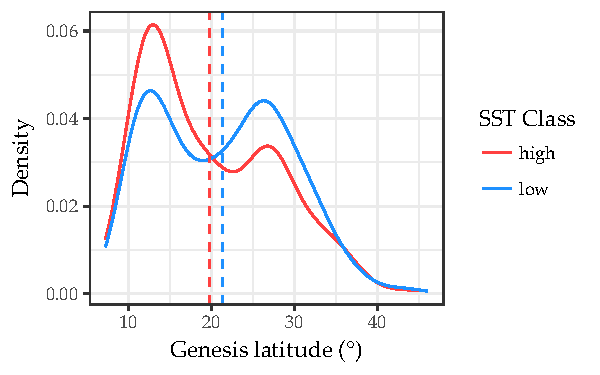
\includegraphics[width=0.5\textwidth]{./images/natl-init-lat}
		\label{fig:images/natl-init-lat}%
		}%
	\subfloat[Distribution of the death latitude]{%
		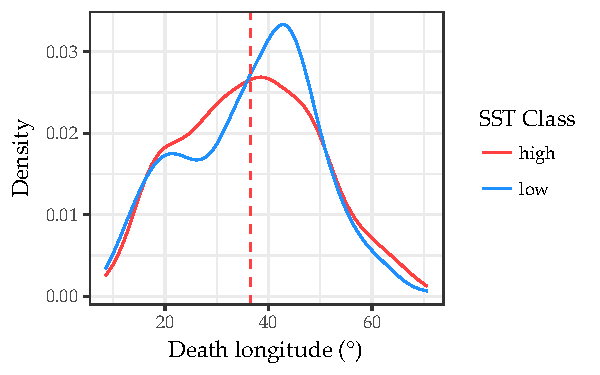
\includegraphics[width=0.5\textwidth]{./images/natl-final-lat}
		\label{fig:images/natl-final-lat}%
		}%
	\caption{Spatial distributions of the geographical position variables of storms for the North Atlantic basin}
	\label{fig:natl-positions}
\end{figure}

\begin{table}[H]
	\centering
	\begin{tabular}{c cc cc}
		\toprule
		\toprule
		SST Class & $\bar{\lambda}_{\text{gen}}$   & $\bar{\phi}_{\text{gen}}$
		          & $\bar{\lambda}_{\text{death}}$ & $\bar{\phi}_{\text{death}}$ \\
		\midrule
		Low       & \num{-59.35 \pm 22.94} & \num{20.84 \pm 7.97} & \num{-59.37 \pm 24.09} & \num{33.08 \pm 12.94} \\
		High      & \num{-58.68 \pm 23.44} & \num{19.47 \pm 7.74} & \num{-59.39 \pm 26.57} & \num{34.72 \pm 13.31} \\
		\bottomrule
	\end{tabular}
	\caption{Summary of the expected values of the geographical position variables of storms for the North Atlantic basin}
	\label{tab:natl-positions}
\end{table}

%-----------------------------------------------------------------
For the Northeast Pacific we have a similar scenario. In \Cref{fig:epac-positions} we can see the distributions of genesis and death positions (longitude and latitde) of the storms, while in \Cref{tab:epac-positions} we can see the expected value of the distributions.

The results suggest show the major difference between low-SST and high-SST years is the location of the genesis of the hurricanes, as it seems to be displaced to the South-East. Contrarily to the North Atlantic, in the Northeast Pacific, there seems to be a slight displacement in the death position for high-SST years to the North-East.

\begin{figure}[H]
	\centering
	\subfloat[Distribution of the genesis longitude]{%
		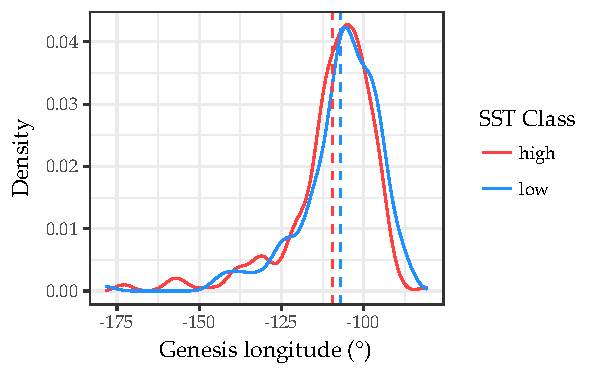
\includegraphics[width=0.5\textwidth]{./images/epac-init-long}
		\label{fig:images/epac-init-long}%
		}%
	\subfloat[Distribution of the death longitude]{%
		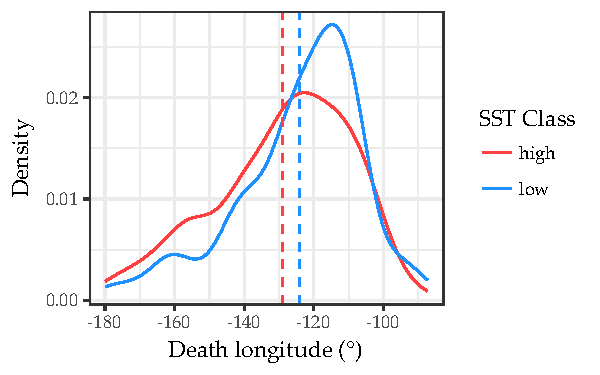
\includegraphics[width=0.5\textwidth]{./images/epac-final-long}
		\label{fig:images/epac-final-long}%
		}%
	\\
	\subfloat[Distribution of the genesis latitude]{%
		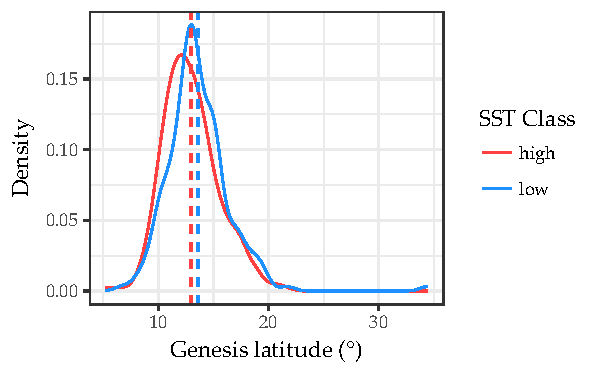
\includegraphics[width=0.5\textwidth]{./images/epac-init-lat}
		\label{fig:images/epac-init-lat}%
		}%
	\subfloat[Distribution of the death latitude]{%
		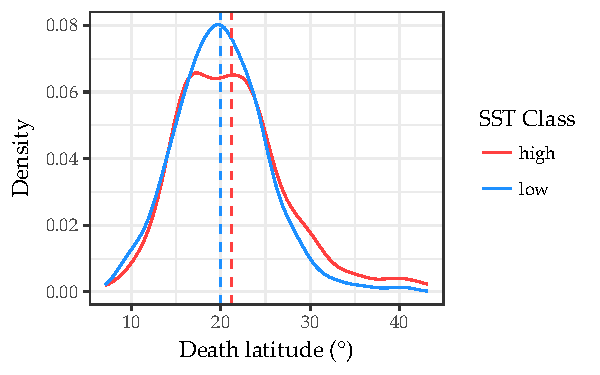
\includegraphics[width=0.5\textwidth]{./images/epac-final-lat}
		\label{fig:images/epac-final-lat}%
		}%
	\caption{Spatial distributions of the geographical position variables of storms for the Northeast Pacific basin}
	\label{fig:epac-positions}
\end{figure}

\begin{table}[H]
	\centering
	\begin{tabular}{c cc cc}
	\toprule
	\toprule
	SST Class & $\bar{\lambda}_{\text{gen}}$   & $\bar{\phi}_{\text{gen}}$
	          & $\bar{\lambda}_{\text{death}}$ & $\bar{\phi}_{\text{death}}$ \\
	\midrule
	Low       & \num{-107.90 \pm 11.98} & \num{13.74 \pm 2.60} & \num{-123.28 \pm 17.34} & \num{19.35 \pm 4.71} \\
	High      & \num{-111.12 \pm 14.92} & \num{13.13 \pm 2.64} & \num{-129.18 \pm 20.11} & \num{20.64 \pm 6.15} \\
	\bottomrule
	\end{tabular}
	\caption{Summary of the expected values of the geographical position variables of storms for the Northeast Pacific basin}
	\label{tab:epac-positions}
\end{table}

\bigskip
